\section{Lecture Six: Stress-Strain Response}
\begin{itemize}
    \item For a \textbf{brittle} material, the slope of the stress-strain graph will be very high and it will have almost no warning before breaking.
    \begin{itemize}
        \item Applications: Piano wires
    \end{itemize}
    \item Other wires, such as \textbf{flossing wires}, which are used to reinforce concrete, there is a different behaviour, where yielding occurs very early.
    \begin{center}
        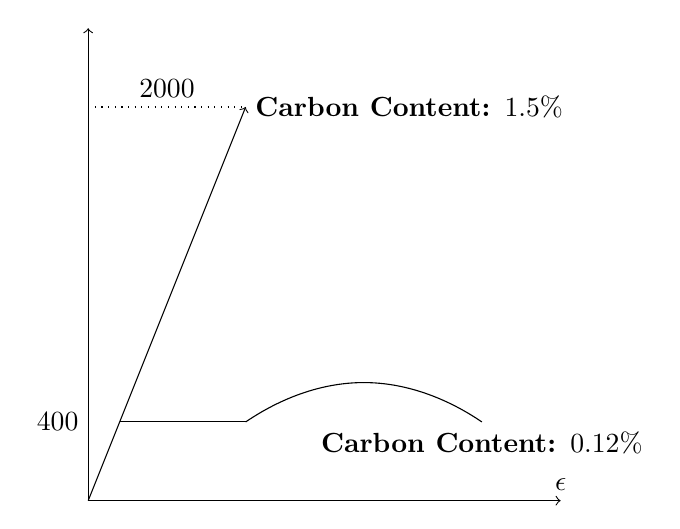
\begin{tikzpicture}
            \coordinate (O) at (0,0);
            \draw[->] (O) -- (6,0) node[above] {$\epsilon$};
            \draw[->] (O) -- (0,6);
            \draw[] (0,1) node[left] {$400\si{\mega\pascal}$};
            \draw[dotted] (0,5) -- (2,5) node[midway,above] {$2000\si{\mega\pascal}$};
            \draw[->] (O) -- (2,5) node[right] {$\textbf{Carbon Content: }1.5\%$};

            \draw[] (0.4,1) -- (2,1);
            \draw[] (3.5,1.5) parabola (2,1);
            \draw[] (3.5,1.5) parabola (5,1) node[below] {$\textbf{Carbon Content: }0.12\%$};
        \end{tikzpicture}
    \end{center}
    \item \textbf{Work} is defined as:
    \begin{equation}
        \text{Work} = \text{Force} \cdot \text{Distance}
        \label{eq:}
    \end{equation}
    and is measured in Joules ($[\si{\joule}]=[\si{\newton\meter}]$) and \textbf{energy} is defined as the capacity to do work
    \item Body fat can store around $40\si{\mega\joule\per\kilogram}$ in body fat, where $7.5\%$ of it can be transferred. One rule of thumb is that one pound of body fat carries you $35$ miles.
    \item Power is the rate at which work is being done. Originally defined as:
    \begin{equation}
        1\text{ HP} = 746\si{\watt}
        \label{eq:}
    \end{equation}
    \item The work, or energy stored in deforming a wire is the area under the curve of the force vs displacement curve. The \textbf{elastic strain energy} gives the maximum recoverable energy, or:
    \begin{equation}
        E=\frac{1}{2}F_\text{max}\Delta_\text{max} = \frac{1}{2}\sigma A \times \epsilon L
        \label{eq:}
    \end{equation}
    The energy density is:
    \begin{equation}
        E/V = \frac{1}{2}\sigma\epsilon
        \label{eq:}
    \end{equation}
    \item The resilience of a material is directly related to its ability to store elastic strain energy.
    \item Some vocabulary terms:
    \begin{itemize}
        \item Weight $[\si{\kilo\newton\per\meter\cubed}]$ - weight density of the material
        \item Stiffness $E[\si{\mega\pascal}]$ - The Young's Modulus: How difficult it is to stretch
        \item Tensile strength $[\si{\mega\pascal}]$- Critical points at which the material starts to yield, or break (ultimate).
        \item Compressive strength  $[\si{\mega\pascal}]$ - yield strength equivalent of tensile strength, except for compressions.
        \item Resilience $[\si{\mega\joule\per\meter\cubed}]$ - maximum energy which a material can absorb per unit volume before experiencing permanent deformations.
        \item Toughness $[\si{\mega\joule\per\meter\cubed}]$ - maximum energy which a material can absorb per unit volume before experiencing permanent deformations.
        \item Ductility is the maximum elongation before it experiences failure.
        \item $\alpha[10^{-6} \si{\per\celsius}]$ - thermal expansion coefficient
    \end{itemize}
\end{itemize}